\section{Notations}
\label{sec:notations}
In this thesis, the following notations are used:
\begin{itemize}
  \item bold lowercase letters ($\vect{a}$, $\vect{b}$, $\vect{c}$) are used to denote vectors;
  \item italic lowercase letters ($a$, $b$, $c$) are used to denote scalars;
  \item bold uppercase letters ($\vect{A}$, $\vect{B}$, $\vect{C}$) are used to denote matrices;
  \item $\vect{a}_{i(j)}$ is the $j$th element of the vector $\vect{a}_i$;
  \item $||\vect{a}||_2$ is the $l^2$-norm of the vector $\vect{a}$, defined as $\sqrt{\sum_{i=1}^{n} a_i^2}$, denoted also as $\norm{a}$ for simplicity;
  \item $||\vect{a}||_n$ is the generic $l^n$-norm of the vector $\vect{a}$, defined as $\sqrt[n]{\sum_{i=1}^{n} \abs{a_i}^n}$;
  \item parenthesis encapsulating an index are used to condense descriptions, for example \quoted{\textbf{$\vect{a}_{i(j)}$ is the force applied to the $i$th ($j$th) step}} means that $\vect{a}_i$ is the force applied to the $i$th step and $\vect{a}_j$ is the force applied to the $j$th step;
  \item date and times are presented in the \gls{iso} 8601 format \cite{iso8601}. \\ For example \texttt{YYYY-MM-DDThh:mm:ss}, where \texttt{T} is the date-time separator;
\end{itemize}

No distinction in notation is made between a vector in the physical sense (applied to a point, with a direction, and a magnitude) and a vector in the mathematical sense (a generic number $\in \mathbb{R}^n $).

As regards the flowcharts, the following symbols shown in \autoref{tab:flowsymbols} are used.


\begin{longtblr}[
  caption = {Symbols used in the flowcharts},
  label = {tab:flowsymbols},
]{
  cell{2}{1} = {t},
  cell{3}{1} = {t},
  cell{5}{1} = {t},
  cell{6}{1} = {t},
  cell{7}{1} = {t},
  hline{1,13} = {-}{0.08em},
  hline{2} = {-}{},
}
\textbf{Symbol} & \textbf{Name} & \textbf{Usage}\\

\includegraphics[scale=1]{images/FlowSymbols/terminator.pdf} & terminator & start or stop the process\\

\includegraphics[scale=1]{images/FlowSymbols/storedData.pdf} & stored data & save some data\\

\includegraphics[scale=1]{images/FlowSymbols/data.pdf} & data & elaborate some data\\

\includegraphics[scale=1]{images/FlowSymbols/process.pdf} & actions & perform automated actions\\

\includegraphics[scale=1]{images/FlowSymbols/document.pdf} & document & read or write a docuument\\
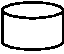
\includegraphics[scale=1]{images/FlowSymbols/database.pdf} & database & perform an action on a database\\

\includegraphics[scale=1]{images/FlowSymbols/display.pdf} & display & report, plot or display a value\\

\includegraphics[scale=1]{images/FlowSymbols/manualInput.pdf} & manual input & request an input from the user\\

\includegraphics[scale=1]{images/FlowSymbols/manualOperation.pdf} & manual operation & request the user to do something\\

\includegraphics[scale=1]{images/FlowSymbols/or.pdf} & or & join flow line\\

\includegraphics[scale=1]{images/FlowSymbols/predefProcess.pdf} & predefined process & run a programmed process
\end{longtblr}